% !TeX root = ../dd.tex
\section{Overview}
The system is a distributed application which follows the microservices architecture paradigm.\\
With the term client we are referring to either a Student or an Educator.\\
Users interact with the system by interfacing with a Single Page App (SPA), served by a Content Delivery Network (CDN).
The site forwards appropriate requests to an API Gateway.
The user is completely unaware of the microservices structure used to operate the system.\\
Each microservice realizes a service useful for the fulfillment of the single functionality that the CKB Platform is to provide.
All requests go through the API Gateway which realizes complex services by sending requests to the several available microservices.\\
The CKB platform can be abstracted into 5 main areas:
\begin{enumerate}

    \item Battles, Tournaments, Teams and Scores
    \item Notifications
    \item Badges
    \item Building and testing
    \item Analysing

\end{enumerate}

\begin{figure}[H]
    \centering
    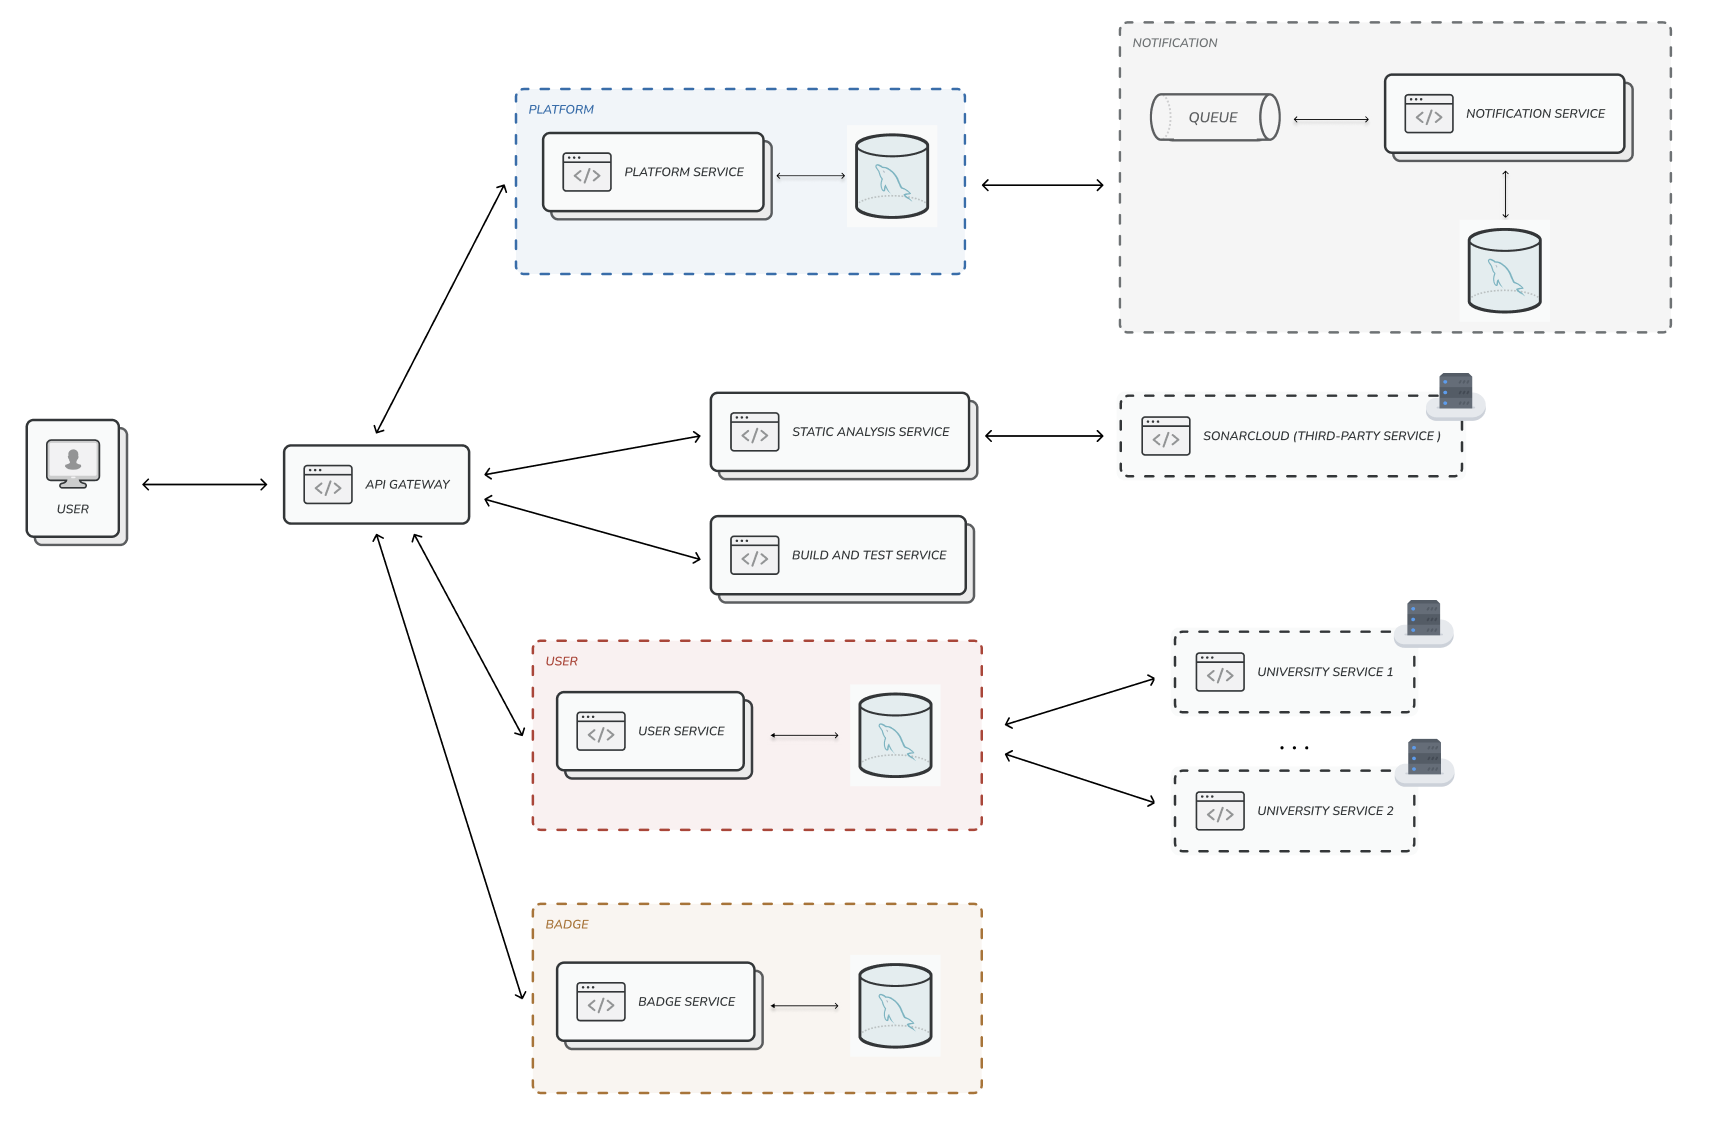
\includegraphics[width=\textwidth]{../images/abstract-system-layout.PNG}
    \caption{Abstract System View}
    \label{fig:Abstract System View}
\end{figure}

These sections contain modules with functionality related to the same domain independent of each other, consequently the areas will be implemented by different microservices ensuring low coupling and high cohesion.\\
The choice to use microservice architecture allows flexibility and scalability because all services can be duplicated by not having to interact with databases shared among microservices that could become bottlenecks of the system.
In particular, the API Gateway is responsible for performing load balancing and being stateless, more or less resources can be dynamically allocated depending on the load of requests that are received.\\
In addition, the components involved in sending notifications, compiling sources, running tests, and analyzing them perform more or less complex operations that may take a few moments of execution time.
Consequently, they will be implemented in such a way as to be asynchronous with the use of message queues avoiding making users wait for a long time (more details in later sections).


\section{Component view}
\begin{adjustbox}{
        max size={\textwidth}{\textheightwithcaption{1}},
        caption={Component view diagram},
        label={fig:Component view diagram},
        figure=H}
    \centering
    \puml{puml/component-view}
\end{adjustbox}

\subsection{Client Components}

\subsection{Server Components}
The server components contain the business logic needed to provide the functionalities of the application to the clients,
by responding to requests made by Client Components as well as perform tasks based on interaction with the external
platforms used by the clients (such as GitHub). There are 5 main components, which corresponds to the main areas identified
above, as well as a few additional components:
\begin{itemize}
    \item \textbf{User Service} {-} implements the authentication as well as keeps track of both students and educators by making
          use of 3rd-party authentication services provided by the institutions.
    \item \textbf{Platform Service} {-} implements all the logic related to creating and managing battles and tournaments, including
          calculating the score and keeping track of the leaderboards
    \item \textbf{Badge Service} {-} implements all the logic related to the evaluation and assignment of badges, including the gathering
          of information needed in order to do that (for example Git or GH metadata such as number of commits by students, etc.)
          as well as the actual evaluation of JavaScript code which gets used by educators in order to express the logic of
          specific badges
    \item \textbf{Build and Test Service} {-} implements the Continuous Integration aspect, by building students projects and
          running them against tests for each push
    \item \textbf{Static Analysis Service} {-} abstracts away the interaction with SonarCloud, the 3rd party service which will
          perform the actual static analysis. While SonarCloud already exposes their own API for interaction, it is cumbersome
          (as it requires registering a webhook \cite{SonarCloudWh}, importing the project from the GH slug \cite{SonarCloudGh},
          specifying the required analysis metrics in a quality profile \cite{SonarCloudQp} and waiting for a response on the hook).
          Therefore, by abstracting it away we can use it much more easily and, additionally, make it much less inconvenient to
          replace it should the need arise.
    \item \textbf{Notification Service} {-} responsible for delivering push notifications
          to client devices using external notification APIs (such as the Web Push API \cite{WebPushApi})
    \item \textbf{Website CDN} {-} responsible for serving the static files of the SPA to the clients
    \item \textbf{API Gateway} {-} responsible for connecting together all microservices, it is the component that provides a REST
          interface externally, which the clients will send requests to, which will be implemented by a series of internal calls
          using gRPC \cite{gRPC} to all the other microservices in order to make responses. The component does not implement a specific
          functionality per se, but is in charge of providing an interface to the clients as well as enforcing the correct usage
          of said interface.
\end{itemize}

\subsection{Data Components}
Server Components make use of 4 distinct DBMSes, each with its own schema.
\begin{itemize}
    \item \textbf{User DB} {-} saves data related to the users of the platform. Its ER schema is not shown
          here as it would depend on the 3rd-party service, but it would at least require for each student and
          educator a unique identifier, as well as human readable identifier to allow users to lookup each other
          (so name and surname or an email). Educators and Students are saved in different tables.
          \pagebreak
    \item \textbf{Platform DB}
          \begin{adjustbox}{
                  max size={\textwidth}{\textheightwithcaption{1}},
                  caption={Platform ER},
                  label={fig:Platform ER},
                  figure=H}
              \centering
              \puml{puml/platform-db}
          \end{adjustbox}
          \pagebreak
    \item \textbf{Badge DB}
          \begin{adjustbox}{
                  max size={\textwidth}{\textheightwithcaption{1}},
                  caption={Badges ER},
                  label={fig:Badges ER},
                  figure=H}
              \centering
              \puml{puml/badges-db}
          \end{adjustbox}
    \item \textbf{Notification DB}
          \begin{adjustbox}{
                  max size={\textwidth}{\textheightwithcaption{1}},
                  caption={Notification ER},
                  label={fig:Notification ER},
                  figure=H}
              \puml{puml/notification-db}
              \centering
          \end{adjustbox}
\end{itemize}
\pagebreak

\section{Deployment view}
\begin{adjustbox}{
        max size={\textwidth}{\textheightwithcaption{1}},
        caption={Deployment view diagram},
        label={fig:Deployment view diagram},
        figure=H}
    \centering
    \puml{puml/deployment-diagram}
\end{adjustbox}

The website is served by a CDN, such as Cloudflare, Amazon CloudFront or Akamai.
This allows to always have the maximum efficiency, regardless of the number of users connected at the same time.

All other microservices are protected by a firewall that allows only HTTPS connections to the API Gateway.
All microservices can be hosted on-premise or in cloud, within a virtual network, such as Amazon VPC \cite{VPC}.
Since the expected workload will not be constant over time (all students study more or less at the same times),
an on-premise architecture would be unused most of the time, resulting in a waste of money.
The best choice is therefore a cloud architecture, such as Amazon EC2 \cite{EC2}, that allows to scale up resources only when really needed.

The API Gateway is stateless and can be implemented with the Spring Cloud Gateway \cite{SpringCloudGateway}.
It is built on top of the Reactor project \cite{Reactor}, which provides a non-blocking API for routing and filtering requests.
This allows to handle high traffic and scale the API Gateway horizontally when necessary.

The Build and Test Service is based on the Jenkins system \cite{Jenkins}.
It is the most CPU-intensive service and should adopt a distributed builds architecture \cite{JenkinsScale}.
One possibility is to have a single Jenkins controller that schedules builds to dedicated build nodes (agents).
Build agents can be dynamically deployed to a new EC2 instance and removed, based on the current workload.\\
If the CKB platform will grow up, an architecture with multiple controllers can be adopted.
For example, the platform can create a Jenkins controller for each tournament.

All other service are implemented as Spring Boot \cite{SpringBoot} applications and they can be deployed to EC2 instances.

The Platform Service, Badge Service, User Service and Notification Service also have their own database.
They use a managed DB service, such as Amazon RDS, that can automatically manage backups and resource scaling.
Each database is in a private subnetwork and it can be accessed only by its corresponding service.

The Notification Service uses RabbitMQ \cite{RabbitMQ} to create a queue where the Platform Service can push messages.
The service will periodically pop messages from the queue with the Spring AMQP project \cite{SpringAMQP} and send them.

\pagebreak

\section{Runtime view}
The following sequence diagrams represent the dynamics of interaction between components.\\
Sequence diagrams from \ref{{RW1}} to \ref{{RW9}} are the realizations of the corresponding use cases in the RASD document.\\
Sequence diagrams from \ref{{RW0.1}} to \ref{{RW0.4}} are common part that have been extracted for simplicity and are not shown in other diagrams.\\
In the first three sequence diagrams, the user could be a student or an educator.

\begin{enumerate}[label=\textbf{RW\arabic*}:,ref=RW\arabic*,leftmargin=1.3cm]
    \item[]
          \begin{enumerate}[label=\textbf{RW\arabic{enumi}.\arabic*}:,ref=RW\arabic{enumi}.\arabic*,leftmargin=0.5cm]
              \labelledsubitem{
                  \textbf{}
                  \begin{adjustbox}{
                          max size={\textwidth}{\textheightwithcaption{1}},
                          caption={User gets list of tournaments},
                          label={fig:User gets list of tournaments},
                          figure=H}
                      \centering
                      \puml{puml/rw0.1}
                  \end{adjustbox}
                  \pagebreak
              }
              \labelledsubitem{
                  \textbf{}
                  \begin{adjustbox}{
                          max size={\textwidth}{\textheightwithcaption{1}},
                          caption={User gets tournament details},
                          label={fig:User gets tournament details},
                          figure=H}
                      \centering
                      \puml{puml/rw0.2}
                  \end{adjustbox}
              }
              \labelledsubitem{
                  \textbf{}
                  \begin{adjustbox}{
                          max size={\textwidth}{\textheightwithcaption{1}},
                          caption={User gets battle details},
                          label={fig:User gets battle details},
                          figure=H}
                      \centering
                      \puml{puml/rw0.3}
                  \end{adjustbox}
                  \pagebreak
              }
              \labelledsubitem{
                  \textbf{}
                  \begin{adjustbox}{
                          max size={\textwidth}{\textheightwithcaption{1}},
                          caption={Notification is sent},
                          label={fig:Notification is sent},
                          figure=H}
                      \centering
                      \puml{puml/rw0.4}
                  \end{adjustbox}
                  This diagram shows the process of sending a notification.
                  The Notification Service will periodically pop from the Notification Queue messages that contains an array of ids of the recipient students.
                  Then the Notification Service will look for each student's endpoint URL (previously registered by clients using the API Gateway)
                  and sends the notifications.
                  \pagebreak
              }
          \end{enumerate}

          \labelleditem{
              \textbf{}
              \begin{adjustbox}{
                      max size={\textwidth}{\textheightwithcaption{1}},
                      caption={Educator creates a new Tournament},
                      label={fig:Educator creates a new Tournament},
                      figure=H}
                  \centering
                  \puml{puml/rw1}
              \end{adjustbox}
              \pagebreak
          }
          \labelleditem{
              \textbf{}
              \begin{adjustbox}{
                      max size={\textwidth}{\textheightwithcaption{1}},
                      caption={Educator creates a new badge},
                      label={fig:Educator creates a new badge},
                      figure=H}
                  \centering
                  \puml{puml/rw2}
              \end{adjustbox}
              \pagebreak
          }
          \labelleditem{
              \textbf{}
              \begin{adjustbox}{
                      max size={\textwidth}{\textheightwithcaption{1}},
                      caption={Educator creates a new Battle for an Existing Tournament},
                      label={fig:Educator creates a new Battle for an Existing Tournament},
                      figure=H}
                  \centering
                  \puml{puml/rw3}
              \end{adjustbox}
              \pagebreak
          }
          \labelleditem{
              \textbf{}
              \begin{adjustbox}{
                      max size={\textwidth}{\textheightwithcaption{1}},
                      caption={Student joins to an existing Tournament by receiving a notification},
                      label={fig:Student joins to an existing Tournament by receiving a notification},
                      figure=H}
                  \centering
                  \puml{puml/rw4}
              \end{adjustbox}
              \pagebreak
          }
          \labelleditem{
              \textbf{}
              \begin{adjustbox}{
                      max size={\textwidth}{\textheightwithcaption{1}},
                      figure=H}
                  \centering
                  \puml{puml/rw5-part1}
              \end{adjustbox}
              \pagebreak
              \begin{adjustbox}{
                      max size={\textwidth}{\textheightwithcaption{1}},
                      caption={Students create a team for a tournament battle},
                      label={fig:Students create a team for a tournament battle},
                      figure=H}
                  \centering
                  \puml{puml/rw5-part2}
              \end{adjustbox}
              \pagebreak
          }
          \labelleditem{
              \textbf{}
              \begin{adjustbox}{
                      max size={\textwidth}{\textheightwithcaption{1}},
                      caption={Student forks the repository},
                      label={fig:Student forks the repository},
                      figure=H}
                  \centering
                  \puml{puml/rw6}
              \end{adjustbox}
              \pagebreak
          }
          \labelleditem{
              \textbf{}
              \begin{adjustbox}{
                      max size={\textwidth}{\textheightwithcaption{2}},
                      caption={Student pushes and triggers automatic evaluation},
                      label={fig:Student pushes and triggers automatic evaluation},
                      figure=H}
                  \centering
                  \puml{puml/rw7}
              \end{adjustbox}
              \pagebreak
          }
          \labelleditem{
              \textbf{}
              \begin{adjustbox}{
                      max size={\textwidth}{\textheightwithcaption{1}},
                      caption={Educator manually evaluates teams},
                      label={fig:Educator manually evaluates teams},
                      figure=H}
                  \centering
                  \puml{puml/rw8}
              \end{adjustbox}
              \pagebreak
          }
          \labelleditem{
              \textbf{}
              \begin{adjustbox}{
                      max size={\textwidth}{\textheightwithcaption{1}},
                      caption={Educator closes a tournament},
                      label={fig:Educator closes a tournament},
                      figure=H}
                  \centering
                  \puml{puml/rw9}
              \end{adjustbox}
              \pagebreak
          }
\end{enumerate}

\section{Component interfaces}
Here the most relevant interfaces exposed by components are described, including all the operations
seen in the previous diagrams:
\begin{itemize}
    \item \textbf{API Gateway}
          \begin{itemize}
              \item \textbf{getListOfTournaments(authToken: String): List<SimpleTournament>}
                    given a valid educator auth token, returns the list of tournaments which he has created
                    or he has permissions to add battles to
              \item \textbf{getTournamentDetails(authToken: String, tournamentId: ID): Tournament}
                    returns the detailed tournament info for the given id
              \item \textbf{getBattleDetails(authToken: String, battleId: ID): Battle}
                    returns the detailed battle info for the given id
              \item \textbf{searchEducator(authToken: String, name: String?, surname: String?, \ldots): ID?}
                    search for an educator matching the given name and/or surname
              \item \textbf{searchStudent(authToken: String, name: String?, surname: String?, \ldots): ID?}
                    search for a student matching the given name and/or surname
              \item \textbf{createTournament(authToken: String, tournamentInfo: NewTournament): ID}
                    create a new tournament with the given info and return its id
              \item \textbf{createBadge(authToken: String, badgeInfo: NewBadge): ID}
                    create a new badge with the given info and return its id
              \item \textbf{createNewBattle(authToken: String, tournementId: ID, battleInfo: Battle): ID}
                    create a new battle with the given info and return its id
              \item \textbf{enrollInTournament(authToken: String, tournementId: ID): void}
                    enroll the student owning the given token in the given tournament
              \item \textbf{createTeam(authToken: String, battleId: ID): ID}
                    create a new team to take part in the given battle and assign the student owning the given token
                    to it, returning the id of the created team
              \item \textbf{invite(authToken: String, newTeamId: ID, invitedStudentId: ID): void}
                    send an invitation for the given team to the invitedStudentId, with the student owning the given token
                    as the invite sender
              \item \textbf{acceptInvitation(authToken: String, invitation: ID): void}
                    accept the given invitation
              \item \textbf{rejectInvitation(authToken: String, invitation: ID): void}
                    reject the given invitation
              \item \textbf{enrollInBattle(authToken: String, teamId: ID): void}
                    enroll the given team in the battle
              \item \textbf{insertRepoSlug(authToken: String, battleId: ID, repo: Slug): void }
                    associate the given GH repository to the team of the student owning the given token for the
                    specified battle
              \item \textbf{newPush(repo: Slug): void }
                    triggered by the GHA on a new push to the specified repository
              \item \textbf{assignGrade(authToken: String, battleId: ID, teamId: ID, grade: Int): void }
                    assign this gradle to the submission of the specified team in the given battle
              \item \textbf{closeTournament(authToken: String, tournamentId: ID): void }
                    close the given tournament
              \item \textbf{closeBattle(authToken: String, battleId: ID): void }
                    close the given battle while it's in its consolidation phase
              \item \textbf{addStudentNotificationEndpoints(authToken: String, endpoint: String): void}
                    add the URL of the notification endpoints of a student
          \end{itemize}
    \item \textbf{User Interface}
          \begin{itemize}
              \item \textbf{validateEducatorToken(authToken: String): ID?}
                    validate that the given token is a valid educator token and return its educator id
              \item \textbf{validateStudentToken(authToken: String): ID?}
                    validate that the given token is a valid student token and return its student id
              \item \textbf{searchEducator(name: String?, surname: String?, \ldots): ID?}
                    search for an educator matching the given name and/or surname
              \item \textbf{searchStudent(name: String?, surname: String?, \ldots): ID?}
                    search for a student matching the given name and/or surname
              \item \textbf{checkEducatorIds(educatorsIds: ID[]): Bool}
                    checks that the given ids are all associated to an existing educator
              \item \textbf{checkStudentId(studentId: ID): Bool}
                    checks that the given id is associated to an existing student
          \end{itemize}
    \item \textbf{Platform Interface}
          \begin{itemize}
              \item \textbf{getListOfTournaments(educatorId: ID): List<SimpleTournament>}
                    given an educator id, returns the list of tournaments which he has created
                    or he has permissions to add battles to
              \item \textbf{getTournamentDetails(tournamentId: ID): Tournament}
                    returns the detailed tournament info for the given id
              \item \textbf{getBattleDetails(battleId: ID): Battle}
                    returns the detailed battle info for the given id
              \item \textbf{createTournament(creatorId: ID, tournamentInfo: NewTournament): ID}
                    create a new tournament with the given info and return its id
              \item \textbf{createNewBattle(tournementId: ID, battleInfo: NewBattle): ID}
                    create a new battle with the given info and return its id
              \item \textbf{enrollInTournament(studentId: ID, tournementId: ID): void}
                    enroll the given student in the given tournament
              \item \textbf{createTeam(battleId: ID, studentId: ID): ID}
                    create a new team to take part in the given battle and assign the student owning the given token
                    to it, returning the id of the created team
              \item \textbf{invite(newTeamId: ID, invitedStudentId: ID): void}
                    send an invitation for the given team to the specified student, with the student owning the given token
                    as the invite sender
              \item \textbf{acceptInvitation(invitation: ID): void}
                    accept the given invitation
              \item \textbf{rejectInvitation(invitation: ID): void}
                    reject the given invitation
              \item \textbf{enrollInBattle(teamId: ID): void}
                    enroll the given team in the battle
              \item \textbf{insertRepoSlug(studentId: ID, battleId: ID, repo: Slug): void }
                    associate the given GH repository to the team of the student owning the given token for the
                    specified battle
              \item \textbf{findBattleAndTeamFor(repo: Slug): {battleId: ID, teamId: ID}? }
              \item \textbf{calculateNewScore(battleId: ID, teamId: ID, testsReport: TestReport, stReport: StaReport): void }
              \item \textbf{assignGrade(battleId: ID, teamId: ID, grade: Int): void }
                    assign this gradle to the submission of the specified team in the given battle
              \item \textbf{closeTournament(tournamentId: ID): void }
                    close the given tournament
              \item \textbf{closeBattle(battleId: ID): void }
                    close the given battle while it's in its consolidation phase
          \end{itemize}
    \item \textbf{Badge Interface}
          \begin{itemize}
              \item \textbf{createBadge(creatorId: ID, badgeInfo: NewBadge): ID}
                    create a new badge with the given info and return its id
              \item \textbf{createVariable(name: String, code: String): void}
                    create a new variable that can be used in badges
              \item \textbf{assignBadges(tournament: Tournament): void}
                    evaluate and assign badges to all the students that took part in the given tournament
          \end{itemize}
    \item \textbf{Notification Interface}
          \begin{itemize}
              \item \textbf{addStudentNotificationEndpoints(studentId: ID, endpoint: String): void}
                    add the URL of the notification endpoints of a student
          \end{itemize}
    \item \textbf{Static Analysis Interface}
          \begin{itemize}
              \item \textbf{buildAndTest(repo: Slug): TestReport}
                    build the given repository, run its tests and produce a report
          \end{itemize}
    \item \textbf{Build and Test Interface}
          \begin{itemize}
              \item \textbf{analyse(repo: Slug): StaReport}
                    run static analysis on the given repository and produce a report
          \end{itemize}
\end{itemize}

Types:
\begin{itemize}
    \item \textbf{ID} {-} a unique identifier for a given object, could be a self-incrementing integer or a UUID (depends on the choosen DBMS)
    \item \textbf{Slug} {-} a String identifying a specific GitHub repository, in the format `<username>/<repository>' as can be seen
          in a GitHub project URL
    \item \textbf{SimpleTournament}
          \begin{lstlisting}
{
    id: ID,
    name: String,
    status: Subscribing | InProgress | Closed,
} 
          \end{lstlisting}
    \item \textbf{Tournament}
          \begin{lstlisting}
{
    id: ID,
    name: String,
    status: Subscribing | InProgress | Closed,
    subscriptionDeadline: DateTime,
    enrolledStudents: { id: ID, name: String, score: Int }[],
    battles: { id: ID }[],
} 
          \end{lstlisting}
    \item \textbf{NewTournament}
          \begin{lstlisting}
{
    name: String,
    subscriptionDeadline: DateTime,
    authorizedEducators: { id: ID },
    badges: { id: ID }[],
} 
          \end{lstlisting}
    \item \textbf{Battle}
          \begin{lstlisting}
{
    name: String,
    description: String,
    status: Registration | Submission | Consolidation | Done,
    minStudents: Int,
    maxStudents: Int,
    registrationDeadline: DateTime,
    submissionDeadline: DateTime,
    requiresManualEvaluation: Bool,
    repo: Slug?,
    teams: { id: ID, students: { id: ID }[], score: Int }[],
} 
          \end{lstlisting}
    \item \textbf{NewBattle}
          \begin{lstlisting}
{
    name: String,
    description: String,
    minStudents: Int,
    maxStudents: Int,
    registrationDeadline: DateTime,
    submissionDeadline: DateTime,
    requiresManualEvaluation: Bool,
    zippedProject: Blob,
    privateProjectFiles: Path[],
    sonarRules: {
        key: String,
        parameters: {
            key: String,
            value: String,
        }[],
    }[],
}
          \end{lstlisting}
          The zippedProject field is a binary blob which contains all project files and tests, both public and private.
          The privateProjectFiles is in charge of defining which files from this zip will be hidden from the students,
          so that educators can specify private tests. Care must be taken by educators so that the project build script
          can also work in the absence of those files. The sonarRules field lists all the rules to be applied by
          SonarCloud when scanning.
    \item \textbf{NewBadge}
          \begin{lstlisting}
{
    title: String,
    condition: String,
} 
          \end{lstlisting}
    \item \textbf{TestReport}
          \begin{lstlisting}
{
    passed: Int,
    failed: Int,
} 
          \end{lstlisting}
    \item \textbf{StaReport}
          \begin{lstlisting}
Map<{ metricName: String }, { score: Int }> 
          \end{lstlisting}
\end{itemize}

\section{Selected architectural styles and patterns}
\begin{description}[leftmargin=0pt]
    \item[Fat client:]
          fat clients allow offering a wide variety of functionalities independent from the central server, as well as
          to move part of the business logic off of the server and into the clients.
          The main advantages it offers are greater decoupling of frontend and backend as well as a better interactive
          experience, especially in conditions where the client is on an unstable network.
          Additionally, with the adoption of a single-page applications, there are many cross-platform frameworks
          which allow to reuse code partially or entirely on multiple platforms.
          The single-page web application can also be served by a dedicated static webserver, as all its interactivity is
          implemented client-side, further reducing the burden on the server by delegating its serving to a CDN, which is
          highly optimized for this specific use case.
    \item[REST API:] an architectural style defined on top of HTTP centered around the definition of a standardized
          set of stateless operations. Its main advantages are its simplicity, its use of widely adopted standards which
          facilitate adoption, and its ease of scalability given by its stateless nature. It allows to have a single API
          interface against which a heterogeneous set of clients can make requests.
    \item[Microservices architecture:]
          an architectural style where a single application is developed as a suite of small services,
          each running in its own process and each dealing with a single bounded context in the target domain. The use of
          this architecture allows us a more fine-grained scaling strategy, as we can clearly select in our system CPU-bound
          services (such as the Build and Test Service) which will need to have many more resources allocated to it compared
          to the rest of the system.
    \item[API Gateway:]
          a mediator which sits between clients and a service being invoked, which allows to implement cross-cutting concerns
          such as authentication mechanism common for all microservices.It also makes it possible to keep track of and locate references to the different instances of microservices.
    \item[RPC:] an interaction style where remote calls resembles procedure call in a local setting. In particular, we have
          choosen to use gRPC and adopt its philosophy, centered around ``coarse-grained message exchange while avoiding the
          pitfalls of distributed objects and the fallacies of ignoring the network'' \cite{gRPCPrinciples}, therefore
          avoiding many of the issues normally stemming from RPC/RMI. Additionally, its support out-of-the-box for many
          languages, load-balancing, blocking \& non-blocking support and HTTP transport make it a perfect fit for use in a
          microservice architecture.
    \item[Pub-sub/Message queueing:] a messaging pattern which allows to obtain a high degree of decoupling among components
          in both space and time: a publisher does not need to know of the existence of a subscriber and can continue to
          operate independently even if there is none. By doing so, asynchronous communication is implemented.
    \item[Tiered architecture:] the separation of the architecture in layers, such as presentation, business and data,
          offers great flexibility, maintainability and scalability. In particular, by separating the business from the data
          and having communication between components always go through a predefined API, we do not have to worry about
          each knowing the internal representation of the others.
    \item[Stateless components:] the use of stateless components, which do not have memory of interactions they have previously
          received, allows to decouple successive calls to services and facilitates the horizontal scaling of the system.
\end{description}

\section{Other design decisions}
\begin{description}[leftmargin=0pt]
    \item[Relational DBMS:]
          a relational database is the traditional choice because of their guarantees given by ACID properties
          enforcing consistency on the data, as well as their fixed schema with well defined entities which fits
          well with the well-defined model we have identified
\end{description}
